L'Information Retrieval rappresenta un campo interdisciplinare che si concentra sulla progettazione e lo sviluppo di metodologie, algoritmi e sistemi finalizzati a recuperare informazioni rilevanti da collezioni di dati eterogenei e spesso imponenti. A differenza dell'indicizzazione tradizionale dei dati, che organizza le risorse in base a criteri predefiniti, l'Information Retrieval mira a fornire agli utenti la capacità di formulare query personalizzate e ottenere risultati coerenti con le loro necessità informative.

Questo processo di recupero dell'informazione si basa su una serie di principi fondamentali. In primo luogo, gli utenti esprimono le loro richieste attraverso query, che possono essere composte da parole chiave, frasi o domande complete. L'Information Retrieval si impegna quindi a interpretare e comprendere le intenzioni sottostanti di queste query, cercando di identificare non solo le corrispondenze letterali, ma anche il contesto e il significato implicito. Successivamente, il sistema di Information Retrieval cerca all'interno della collezione di dati e documenti indicizzati per individuare quelli che meglio soddisfano le richieste dell'utente.

L'elemento chiave nell'Information Retrieval è la valutazione della rilevanza. Ogni documento recuperato viene valutato in base alla sua pertinenza rispetto alla query dell'utente. Tuttavia, la rilevanza è spesso un concetto sfumato e soggettivo, poiché può variare in base al contesto, all'utente e alle circostanze. Di conseguenza, molti sistemi di Information Retrieval utilizzano tecniche di ranking per ordinare i risultati in modo da presentare quelli più rilevanti o probabilmente interessanti all'utente in cima alla lista.

Un aspetto cruciale dell'Information Retrieval è la necessità di bilanciare l'efficienza e l'accuratezza. I sistemi di ricerca devono essere in grado di gestire grandi volumi di dati e rispondere rapidamente alle query degli utenti, garantendo al contempo che i risultati siano altamente pertinenti. Questa sfida ha portato allo sviluppo di algoritmi di ricerca e tecniche di indicizzazione sempre più sofisticati, che sfruttano modelli matematici, apprendimento automatico e processamento del linguaggio naturale per migliorare la qualità del recupero delle informazioni.

Nella figura~\ref{fig:comefunzir} si può osservare come tutto parta dall'utente che richiede una informazione tramite una query, tale query può essere espressa in varie forme come costraints da rispettare oppure una frase in linguaggio naturale, la query arriva al sistema IR che tramite gli indici precedentemente creati trova i documenti più rilevanti e fornisce un feedback all'utente. 
\begin{figure}[H]
    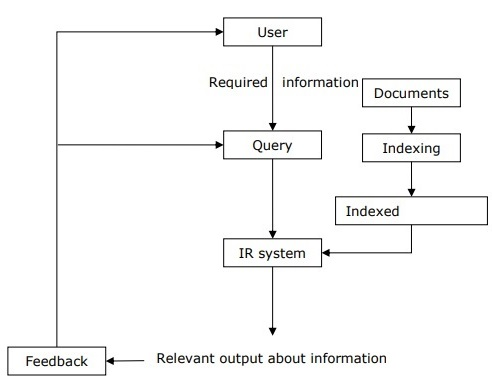
\includegraphics{images/comefunzionair.jpg}
    \caption{Come funziona generalmente un sistema di Information Retrieval}
    \label{fig:comefunzir}
\end{figure}

In sintesi, l'Information Retrieval svolge un ruolo cruciale nella navigazione dell'oceano di dati digitali, fornendo strumenti e metodologie per individuare e accedere alle informazioni desiderate. Questo campo continua a evolversi in risposta alla crescente complessità delle risorse informative e alle mutevoli aspettative degli utenti, spingendo verso l'adozione di approcci sempre più innovativi e tecnologicamente avanzati.
